\chapter{Design}

\section{Overall System Design}

\subsection{Short description of the main parts of the system}

\subsection{System flowcharts showing an overview of the complete system}

\section{User Interface Designs}

\section{Program Structure}

\subsection{Top-down design structure charts}

\subsection{Algorithms in pseudo-code for each data transformation process}

\subsection{Object Diagrams}

\subsection{Class Definitions}

\section{Prototyping}

\section{Definition of Data Requirements}

\subsection{Identification of all data input items}

\subsection{Identification of all data output items}

\subsection{Explanation of how data output items are generated}

\subsection{Data Dictionary}

\subsection{Identification of appropriate storage media}

\section{Database Design}

\subsection{Normalisation}

\newpage

\subsubsection{ER Diagrams}

\begin{figure}[H]
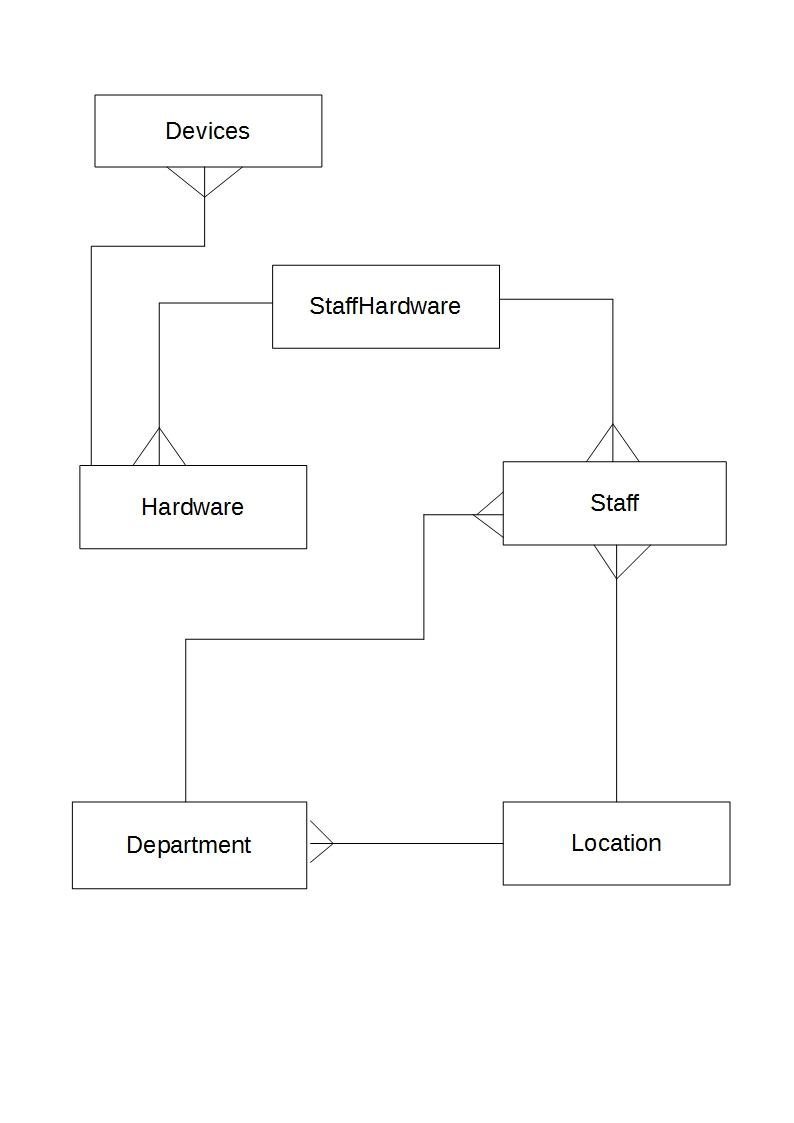
\includegraphics[width=\textwidth]{ERNormalisedDiagram.jpg}
\end{figure}


\subsubsection{Entity Descriptions}

\begin{center}
Staff  (\underline{StaffID}, FirstName, LastName, JobTitle, \textit{DepartmentID},\\ \textit{ LocationID})
\end{center}

\

\begin{center}
Hardware  (\underline{HardwareID}, \textit{Device}, HardwareMake, HardwareModel,\\ HardwareCost, HardwareWarranty, HardwareWarrantyPeriod,\\ HardwareSerialNumber, HardwareIMEINumber, \\HardwarePhoneNumber)
\end{center}

\

\begin{center}
Device  (\underline{Device})
\end{center}

\

\begin{center}
StaffHardware  (\underline{ StaffID}, \underline{ HardwareID},PurchaseDate)
\end{center}

\

\begin{center}
Department  (\underline{DepartmentID}, DepartmentName)
\end{center}

\

\begin{center}
Location  (\underline{LocationID}, LocationName, LocationAddrLine1, LocationAddrLine2, LocationAddrLine3)
\end{center}



\subsubsection{1NF to 3NF}

\begin{figure}[H]
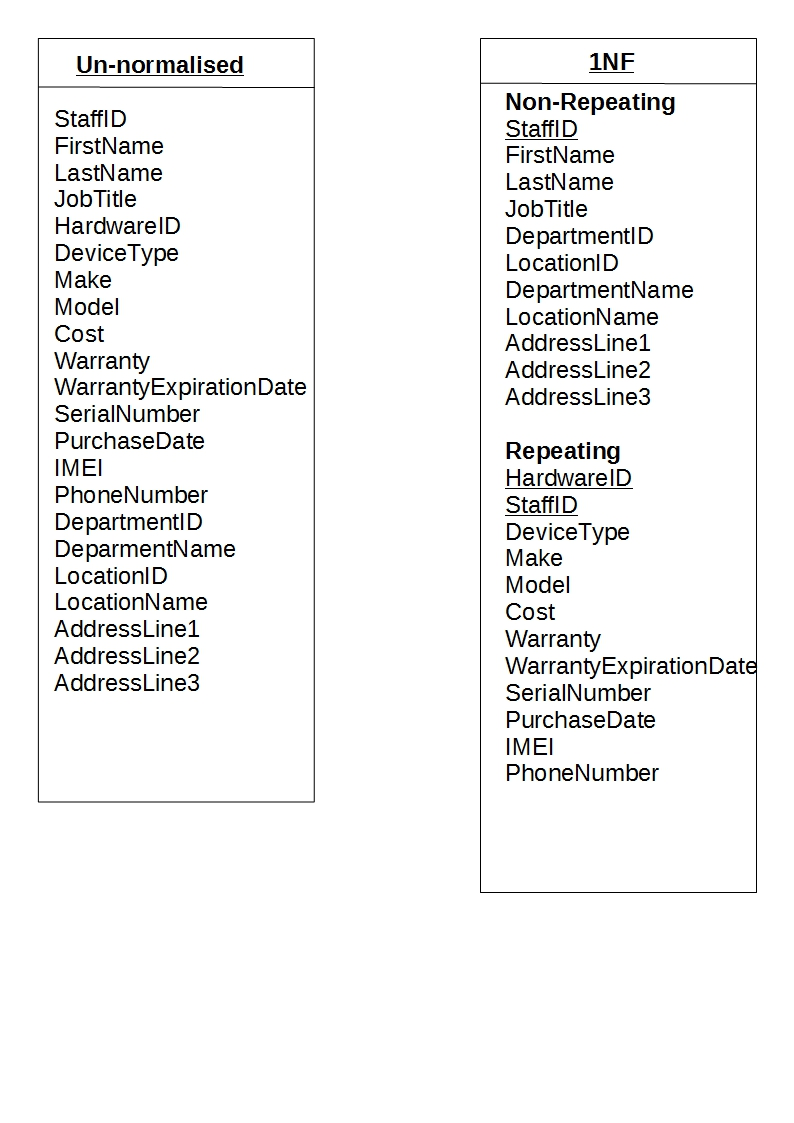
\includegraphics[width=\textwidth]{UNF&1NF.jpg}
\end{figure}

\begin{figure}[H]
\includegraphics[width=\textwidth]{2NF.jpg}
\end{figure}

\begin{figure}[H]
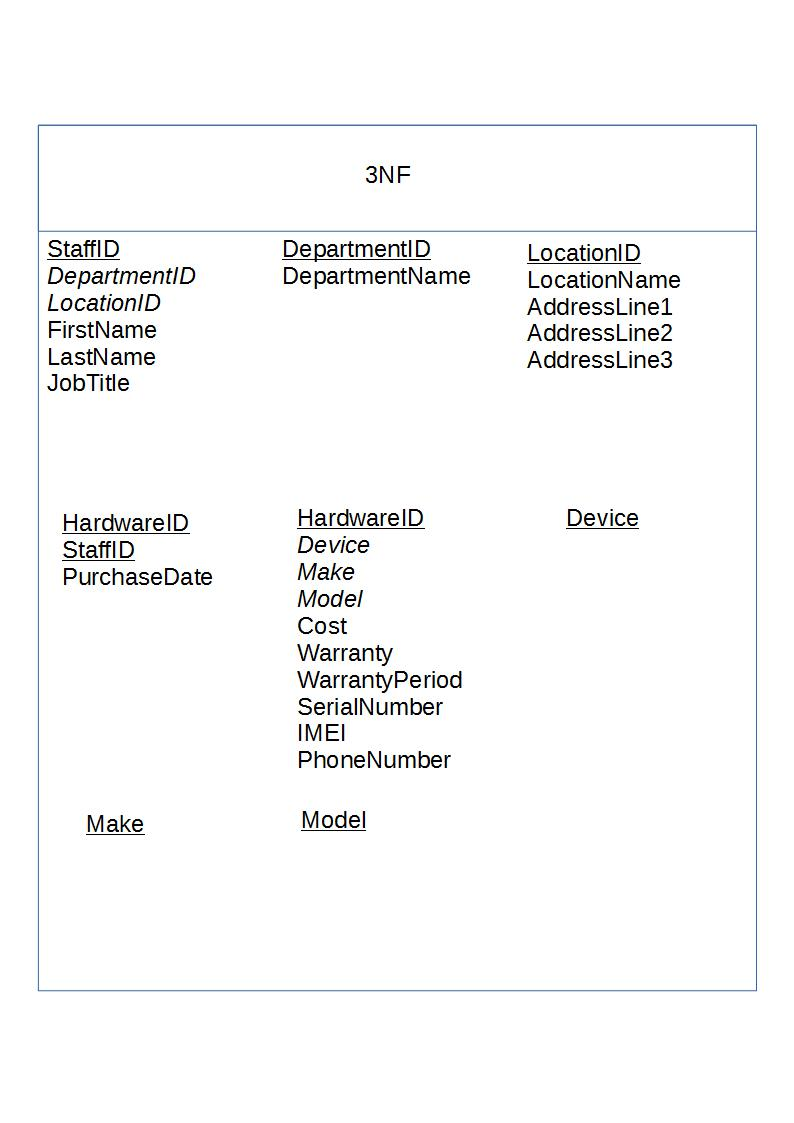
\includegraphics[width=\textwidth]{3NF.jpg}
\end{figure}

\begin{center}
\begin{tabular}{|p{6cm}|p{5cm}|}
\hline
\textbf{SQL}      & \textbf{Description} \\ \hline
"""create table Staff(\

   StaffID INTEGER,\

   FirstName TEXT,\

   LastName TEXT,\

   JobTitle TEXT,\

   DepartmentID INTEGER,\

   LocationID INTEGER,\

   PRIMARY KEY(StaffID))\

   FOREIGN KEY(DepartmentID) \

   REFERENCES Department(DepartmentID)\

   FOREIGN KEY(LocationID) \

   REFERENCES Location(LocationID)) """                         & This SQL statement will create a new table called Staff with the attributes - StaffID, FirstName, LastName, JobTitle, DepartmentID, LocationID, The primary key is StaffID and the foreign keys are DepartmentID and LocationID                       \\ \hline

"""insert into\

Staff(FirstName,LastName, JobTitle, DepartmentID) values
(‘{0}’,’{1}’,’{2}’,'{3}')
""".format(FirstName, LastName, JobTitle, DepartmentID) & This SQL statement will add 3 new records to the database. In this example it is eneterng a new staff record with attributes: FirstName, LastName, JobTitle and DepartmentID \\ \hline

"""delete from Staff\

where StaffID = ‘{3}’\

""".format(StaffID) & This statement will delete the staff member from the Staff table with the StaffID of {3} \\ \hline

\end{tabular}
\end{center}

\section{Security and Integrity of the System and Data}

\subsection{Security and Integrity of Data}

\subsection{System Security}

\section{Validation}

\section{Testing}

\begin{landscape}
\subsection{Outline Plan}

\begin{center}
    \begin{tabular}{|p{2cm}|p{5cm}|p{5cm}|p{4cm}|}
        \hline
        \textbf{Test Series} & \textbf{Purpose of Test Series} & \textbf{Testing Strategy} & \textbf{Strategy Rationale}\\ \hline
        Example & Example & Example & Example \\ \hline
    \end{tabular}
\end{center}

\subsection{Detailed Plan}

\begin{center}
    \begin{longtable}{|p{1.5cm}|p{2.5cm}|p{2.5cm}|p{2cm}|p{2cm}|p{2cm}|p{2cm}|p{2cm}|}
        \hline
        \textbf{Test Series} & \textbf{Purpose of Test} & \textbf{Test Description} & \textbf{Test Data} & \textbf{Test Data Type (Normal/ Erroneous/ Boundary)} & \textbf{Expected Result} & \textbf{Actual Result} & \textbf{Evidence}\\ \hline
        Example & Example & Example & Example & Example & Example & Example & Example \\ \hline
    \end{longtable}
\end{center}
\end{landscape}